\documentclass[../main.tex]{subfiles}

\begin{document}
	\section{Definizione}
	\label{sec:trasformata_laplace}
		Operazione che consente di associare in modo \underline{biunivoco} ad una funzione $ f(t):\left[ 0^{-}, + \infty \right] $ un altra funzione $ F(s) $ a valori complessi $ s = \sigma + j\omega \quad \sigma=\Re(s), \omega=\Im(s) $.\\
		\linebreak
		Se l'integrale $ \int_{0^{-}}^{+\infty}f(t)e^{-st} \mathrm{d}t $ esiste (calcolabile finito), allora $f(t)$ \'e Laplace-trasformabile:
		\[ 
			\Lbrace{f(t)} = F(s) = \LaplDef{f(t)}{s}{t}
		\]
		
		\begin{definition}			
			Si definisce \textbf{ascissa di convergenza} per la trasformata di Laplace di una funzione $ f(t) $ la quantit\'a:
			\[
				\bar{\sigma} \in \R \qquad \bar{\sigma} = inf\left\lbrace \Re{(s)} \colon \exists F(s) = \Lbrace{f(t)} \right\rbrace
			\]
		\end{definition}
		In parole povere si prendono tutti i numeri complessi per cui esiste la trasformata di Laplace. Quindi $ \bar{\sigma} $ \'e l'estremo inferiore di questo insieme (non \'e detto che sia anche il minimo).
		\begin{figure}[H]
			\centering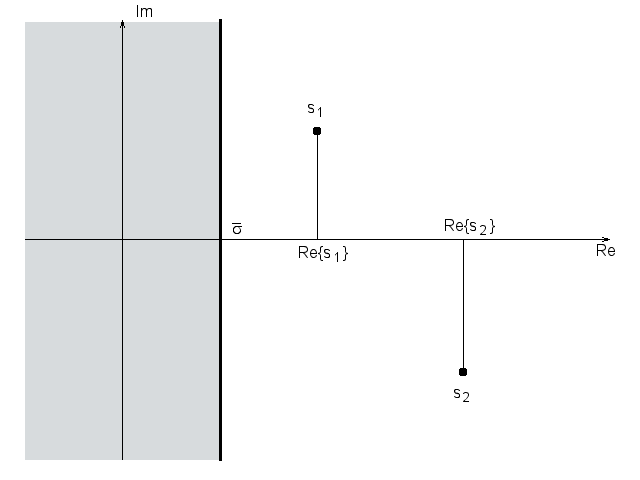
\includegraphics[width=.3\textwidth]{trasformata_laplace/ascissa_convergenza}
			\caption{Nel semipiano grigio la trasformata non esiste}
		\end{figure}
		
		\paragraph{Teorema 1} Se la trasformata di Laplace esiste per qualche $ s=\bar{s} $, allora essa esiste anche $ \forall s\ \text{tale che}\ \Re(s) > \Re(\bar{s}) $.
		
		In pratica l'ascissa di convergenza definisce il limite a destra del quale la trasformata esiste sempre.
		
		\paragraph{Teorema 2} La trasformata di Laplace \'{e} \textbf{analitica} $ \forall s\ \text{tale che}\ \Re(s) > \bar{\sigma} $. Analitica significa che \'e continua e derivabile $ \infty $ volte.
		
		In pratica, se una $ f $ non \'e continua n\'e derivabile in nessun punto, la sua trasformata lo \'e comunque: \'e pi\'u facile lavorare con quest'ultima.
		
	\section{Propriet\'{a}}
	\subsection{Linearit\'{a}}
	\label{sec:linear}
		\[
			\Lapl{f_{1}(t)}{F_{1}(t)} \qquad\qquad \Lapl{f_{2}(t)}{F_{2}(t)}
		\]
		\[
			\Rightarrow\qquad \Lapl{f(t)=\alpha f_{1}(t) + \beta f_{2}(t)}{F(s)=\alpha F_{1}(s) + \beta F_{2}(s)}
		\]
		\paragraph{Dimostrazione}
		\begin{align*}
			\Lbrace{f(t)} = F(s) &= \LaplDef{\big( \alpha f_{1}(t) + \beta f_{2}(t) \big)}{s}{t} =
			\\
			&= \alpha \LaplDef{f_{1}(t)}{s}{t} + \beta \LaplDef{f_{2}(t)}{s}{t} = \alpha F_{1}(s) + \beta F_{2}(s)
		\end{align*}

	\subsection{Traslazione in t}
	\label{sec:trasl_t}
		\[
			\Lapl{f(t)}{F(s)} \quad\Rightarrow\quad \Lapl{f(t-T) \cdot \gr[t-T]}{e^{-sT}F(s)}
		\]
		\paragraph{Dimostrazione}
		chiamiamo $ \bar{f}(t) = f(t-T) \cdot \gr[t-T] $ (con il gradino non consideriamo tutto ci\'{o} che accade prima di $ T $, altrimenti la trasformata sarebbe stata diversa e avrebbe incluso anche il tratto $ (-\infty,T) $).
		\begin{align*}
			\Lbrace{\bar{f}(t)} &= \LaplDef{\bar{f}(t)}{s}{t} = \int_{0^{-}}^{T^{-}} \bar{f}(t) e^{-st} \mathrm{d}t + \int_{T^{-}}^{+ \infty} \bar{f}(t) e^{-st} \mathrm{d}t =
			\\
			&= 0+ \int_{T^{-}}^{+ \infty} f(t-T) \cdot 1 \cdot e^{-st} \mathrm{d}t=
			&&\text{il gradino vale 1 in } (T^{-},+ \infty)
			\\
			&= \int_{0^{-}}^{+ \infty} f(\tau) e^{-s(\tau+T)} \mathrm{d}\tau = &&\text{cambiamento di variabile} \quad \tau=t-T
			\\
			&= e^{-sT} \LaplDef{f(\tau)}{s}{\tau} = e^{-sT} F(s)
		\end{align*}
	
	\subsection{Traslazione in s}
		\label{sec:trasl_s}
		\[
			\Lapl{f(t)}{F(s)} \quad \Rightarrow \quad \Lapl{e^{at}f(t)}{F(s-a)}
		\]
		\paragraph{Dimostrazione}
		chiamo $ \tilde{f}(t) = e^{at} f(t) $:\\
		\[
			\Lbrace{\tilde{f}(t)} = \LaplDef{\tilde{f}(t)}{s}{t} = \LaplDef{e^{at}f(t)}{s}{t} = \int_{0^{-}}^{+ \infty} f(t) e^{-(s-a)t} \mathrm{d}t = F(s-a)
		\]
	%
	\subsection{Derivata in t}
		\label{sec:deriv_t}
		\[
			\Lapl{f(t)}{F(s)} \quad \Rightarrow \quad \Lapl{\dot{f}(t)}{sF(s)-f(0^{-})}
		\]
		\paragraph{Dimostrazione}
		\begin{align*}
			\Lbrace{\dot{f}(t)} &= \LaplDef{\dot{f}(t)}{s}{t} \quad \rightarrow \text{Integro per parti} \rightarrow \left( \int \dot{f}(x)g(x)\mathrm{d}x = f(x)g(x) - \int f(x) \dot g(x) \mathrm{d}x \right)
			\\
			&= \left[ f(t)e^{-st} \right]_{0^{-}}^{+\infty} - \LaplDef{f(t) \cdot (-s) \cdot}{s}{t} =
			\\
			&= 0 - f(0^{-}) + s \LaplDef{f(t)}{s}{t} = sF(s)-f(0^{-})
		\end{align*}
	%
	\subsection{Derivata n-esima in t}
		\label{sec:deriv_n_t}
		\begin{itemize}
			\item $ n=1 $
				\[
					\Lapl{g(t)=\dot{f}(t)}{G(s) = sF(s) - f(0^{-})}
				\]
			\item $ n=2 $
				\[
					\Lapl{\dot{g}(t) = \ddot{f}(t)}{s \cdot G(s) - g(0^{-})} =
				\]
				per la propriet\'a di \hyperref[sec:deriv_t]{derivata in t}:
				\[
					= \quad s \cdot \left[ sF(s) - f(0^{-}) \right] - \dot{f}(0^{-})
				\]
				\[
					\Rightarrow\quad \Lapl{\ddot{f}(t)}{s^2 F(s) - s f(0^{-}) - \dot{f}(0^{-})}
				\]
			\item $ n=3 $
				\[
					\Lapl{\frac{\mathrm{d^3}}{\mathrm{d}t^3}f(t)}{s^3 F(s) - s^2 f(0^{-}) - s f^{(1)}(0^{-}) - f^{(2)}(0^{-})}
				\]
			\item $ n $
				\[
					\begin{aligned}
						\Lapl{\frac{\mathrm{d^n}}{\mathrm{d}t^n}f(t)}{&s^n F(s) - s^{n-1} f(0^{-}) - s^{n-2} f^{(1)}(0^{-}) -\ _{\dots}\ - s f^{(n-2)}(0^{-}) - f^{(n-1)}(0^{-})} =
						\\
						&= s^n F(s) - \sum_{k = 1}^{n} s^{n-k} f^{(k - 1)}(0^{-})
					\end{aligned}
				\]
		\end{itemize}
	
	\subsection{Integrale in t}
		\label{sec:int_t}
		\[
			\Lapl{\int_{0^{-}}^{t} f(\tau) \mathrm{d}\tau}{\frac{1}{s} F(s)}
		\]
		\paragraph{Dimostrazione}
		\[
			g(t) = \int_{0^{-}}^{t} f(\tau) \mathrm{d}\tau, \qquad \dot{g}(t) = f(t), \qquad g(0) = 0
		\]
		Per la propriet\'{a} di \hyperref[sec:deriv_t]{derivata in t}:
		\[
			F(s) = \Lbrace{f(t)} = \Lbrace{\dot{g}(t)} = s \cdot \Lbrace{g(t)} - g(0^{-}) = s \cdot G(s) - 0 \quad \Rightarrow \quad G(s) = \frac{1}{s} F(s)
		\]
		
	\subsection{Derivata in s}
		\label{sec:deriv_s}
		\begin{align*}
			\Lapl{t \cdot f(t)}{&- \der{}{s} F(s)}\\
			\Lapl{t^n \cdot f(t)}{&(-1)^n \frac{\mathrm{d}^n}{\mathrm{d}s^n} F(s)}
		\end{align*}
		\paragraph{Dimostrazione $ n=1 $}
		dalla \hyperref[sec:trasformata_laplace]{definizione} di trasformata di Laplace:
		\[
			\der{}{s} F(s) = \der{}{s} \LaplDef{f(t)}{s}{t} =
		\]
		Uso la regola di derivazione sotto segno di integrale:
		\[
			= \LaplDef{f(t) \cdot \pder{}{s}}{s}{t} = \LaplDef{f(t) \cdot (-t) \cdot}{s}{t} = - \LaplDef{t \cdot f(t) \cdot }{s}{t}=\Lbrace{t \cdot f(t)}
		\]

	\section{Trasformate di funzioni notevoli}
	\subsection{Impulso}
		\label{sec:trasf_impulso}
		Dalla \hyperref[sec:trasformata_laplace]{definizione} di trasformata di Laplace:
		\[
			\Lbrace{\delta (t)} = \LaplDef{\delta (t)}{s}{t} = \int_{0^{-}}^{+ \infty} \delta(t) \cdot 1\ \mathrm{d}t = 1
		\]

	\subsection{Doppietto}
		\label{sec:trasf_doppietto}
		Per la propriet\'{a} di \hyperref[sec:deriv_t]{derivata in t}:
		\begin{align*}
			\Lapl{\dot{\delta}(t)}{&s \cdot \Lbrace{\delta(t)} - \delta(0^-) = s}
			\\
			\Lapl{\delta^{(n)}(t)}{&s^n} \qquad \text{se tutte le condizioni iniziali sono nulle}
		\end{align*}

	\subsection{Gradino}
		\label{sec:trasf_gradino}
		Calcoliamolo in due metodi differenti:
		\begin{enumerate}
			\item Utilizziamo la \hyperref[sec:trasformata_laplace]{definizione} di trasformata di Laplace:
			\[
				\LaplDef{\gr}{s}{t} = \LaplDef{}{s}{t} = -\frac{1}{s}\ \left[ e^{-st} \right]_{0^-}^{+ \infty} = -\frac{1}{s} (-1) = \frac{1}{s}
			\]
			\item \'{E} l'integrale del gradino, quindi possiamo utilizzare la propriet\'{a} di \hyperref[sec:int_t]{integrazione in t}:
			\[
				\gr = \int_{0^-}^{t} \delta(\tau) \mathrm{d}\tau
			\]
			\[
				\Rightarrow\quad \Lapl{\gr}{\frac{1}{s}\ \Lbrace{\delta(t)} = \frac{1}{s}}
			\]
		\end{enumerate}

	\subsection{Rampa}
		\label{sec:trasf_rampa}
		\'{E} l'integrale del gradino, quindi utilizziamo la propriet\'{a} di \hyperref[sec:int_t]{integrazione in t}:
		\begin{align*}
			\Lapl{t \cdot \gr}{&\frac{1}{s} \cdot \Lbrace{\gr}} = \frac{1}{s^2}
			\intertext{Generalizziamo per il grado n:}
			\Lapl{t^n \cdot \gr}{&\frac{n!}{s^{n+1}}}
		\end{align*}

	\subsection{Esponenziale}
		\label{sec:trasf_esponenziale}
		\[
			\Lapl{e^{\sigma t} \cdot \gr}{\frac{1}{s-\sigma}}
		\]

	\subsection{Alcune $f$ composte: Polinomio ed Esponenziale}
		\begin{itemize}
			\item $ n = 1 $: chiamo $ t \cdot e^{\sigma t} \cdot \gr = t \cdot f(t) $
				\begin{align*}
					\intertext{Per la propriet\'{a} di \hyperref[sec:deriv_s]{derivazione in s}:}
					\Lapl{t \cdot f(t)}{&(-1) \der{}{s} F(s)}
					\\
					\Rightarrow\quad \Lapl{f(t) = e^{\sigma t} \cdot \gr}{&F(s) = \frac{1}{s-\sigma}}
					\\
					\Rightarrow \quad \Lapl{t \cdot e^{\sigma t} \cdot \gr}{&(-1) \der{}{s} \frac{1}{s-\sigma}} = (-1) \frac{-1}{(s-\sigma)^2} = \frac{1}{(s-\sigma)^2}
				\end{align*}
			\item $ n $: chiamo  $ f(t) = t^n \cdot \gr $\\
				per la presenza dell'esponenziale sto effettuando una \hyperref[sec:trasl_s]{traslazione in s}:
				\[
					\Lapl{e^{\sigma t} f(t)}{F(s-\sigma)} =  \frac{n!}{(s-\sigma)^{n+1}}
				\]
		\end{itemize}

	\subsection{Seno}
		\label{sec:trasf_seno}
		Scriviamo il seno attraverso la rappresentazione di Eulero dei numeri complessi:
		\begin{align*}
			\Lbrace{\sin(wt) \gr} &= \Lbrace{\frac{e^{jwt} - e^{-jwt}}{2j} \gr} =
			\\
			&= \frac{1}{2j} \left[ \Lbrace{e^{jwt} \gr} - \Lbrace{e^{-jwt} \gr} \right]= \qquad &&\text{per linearit\'{a}}
			\\
			&= \frac{1}{2j} \left[ \frac{1}{s-jw} - \frac{1}{s-(-jw)} \right] = \qquad &&\text{traslazione in s}
			\\
			&= \frac{1}{2j} \frac{s+jw-s+jw}{s^2+w^2} = \frac{w}{s^2+w^2}
		\end{align*}

	\subsection{Coseno}
		\label{sec:trasf_coseno}
		\begin{align*}
			\Lbrace{\cos(wt) \gr} &= \Lbrace{\frac{e^{jwt} + e^{-jwt}}{2} \gr} =
			\\
			&= \frac{1}{2} \left[ \Lbrace{e^{jwt} \gr} + \Lbrace{e^{-jwt} \gr} \right] =
			\\
			&= \frac{1}{2} \left[ \frac{1}{s+jw} + \frac{1}{s-jw} \right] =
			\\
			&= \frac{1}{2} \left[ \frac{s-jw+s+jw}{s^2+w^2} \right] = \frac{s}{s^2+w^2}
			\\
		\end{align*}

	\subsection{Seno e Coseno (2)}
		Gli stessi risultati possono essere ottenuti sfruttando la propriet\'{a} di \hyperref[sec:deriv_t]{derivazione in t}.\\
		\rule{\linewidth}{0.4pt}
		Ad esempio partiamo dal seno:
		\[
			\sin(wt) \quad \xrightarrow{\der{}{t}} \quad w \cos(wt) \quad \xrightarrow{\der{}{t}} \quad -w^2 \sin(wt)
		\]
		Conosciamo la trasformata della funzione seno:
		\[
			\Lbrace{\sin(wt)} = \frac{w}{s^2+w^2}
		\]
		Calcoliamo la trasformata della sua derivata:
		\[
			w \cos(wt) = \der{}{t} \sin(wt) \quad\Rightarrow\quad \Lbrace{w \cos(wt)} = \Lbrace{\der{}{t} \sin(wt)}
		\]
		\[
			\Lbrace{\der{}{t} \sin(wt)} = s \frac{w}{s^2+w^2} - \sin(w\ 0^-) = \frac{sw}{s^2+w^2}
		\]
		Poich\'{e} la trasformata di Laplace \'{e} lineare (\ref{sec:linear}) otteniamo la stessa trasformata del coseno calcolata in precedenza.
		\[
			\Rightarrow \quad \frac{1}{w} \cdot \Lbrace{w\cos(wt)} = \frac{sw}{s^2+w^2} \cdot \frac{1}{w} = \frac{s}{s^2+w^2}
		\]
		Calcoliamo la trasformata della derivata seconda del seno:
		\[
			-w^2 \sin(wt) = \der{}{t} w\cos(wt) \quad\Rightarrow\quad \Lbrace{-w^2 \sin(wt)} = \Lbrace{\der{}{t} w\cos(wt)}
		\]
		\[
			\Lbrace{\der{}{t} w\cos(wt)} = s \frac{sw}{s^2+w^2} - w\cos(w\ 0^-) = \frac{s^2w}{s^2+w^2} - w = \frac{-w^3}{s^2+w^2}
		\]
		\[
			\Rightarrow \quad \left( - \frac{1}{w^2} \right) \cdot \Lbrace{-w^2 \sin(wt)} = \left[ \frac{-w^3}{s^2+w^2} \right] \cdot \left( - \frac{1}{w^2} \right) = \frac{w}{s^2+w^2}
		\]
		\rule{\linewidth}{0.4pt}
		Analogamente partendo dal coseno:
		\[
			\cos(wt) \quad \xrightarrow{\der{}{t}} \quad -w\sin(wt) \quad \xrightarrow{\der{}{t}} \quad -w^2\cos(wt)
		\]
		Calcoliamo la trasformata della sua derivata:
		\[
			-w\sin(wt) = \der{}{t} \cos(wt) \quad\Rightarrow\quad \Lbrace{-w\sin(wt)} = \Lbrace{\der{}{t} \cos(wt)}
		\]
		\[
			\Lbrace{\der{}{t} \cos(wt)} = s \frac{s}{s^2+w^2} - \cos(w\ 0^-) = \frac{s^2}{s^2+w^2} - 1
		\]
		\[
			\Rightarrow \quad -\frac{1}{w} \cdot \Lbrace{-w\sin(wt)} = \left[ \frac{s^2}{s^2+w^2} - 1 \right] \cdot \left( -\frac{1}{w}\right) = \left[ \frac{s^2-s^2-w^2}{s^2+w^2} \right] \cdot \left( -\frac{1}{w}\right) = \frac{w}{s^2+w^2}
		\]
		Calcoliamo la trasformata della derivata seconda del coseno:
		\[
			-w^2 \cos(wt) = \der{}{t} \left[ -w\sin(wt) \right] \quad\Rightarrow\quad \Lbrace{-w^2 \cos(wt)} = \Lbrace{\der{}{t} \left[ -w\sin(wt) \right]}
		\]
		\[
			\Lbrace{\der{}{t} \left[ -w\sin(wt) \right]} = s \left[ \frac{s^2}{s^2+w^2} - 1 \right] - \left[ -w\sin(w\ 0^-) \right] = s \left[ \frac{s^2}{s^2+w^2} - 1 \right]
		\]
		\[
			\Rightarrow \quad \left( - \frac{1}{w^2} \right) \cdot \Lbrace{-w^2 \cos(wt)} = s \left[ \frac{s^2}{s^2+w^2} - 1 \right] \left[ - \frac{1}{w^2} \right] = \left[ \frac{\not{s^2}-\not{s^2}-w^2}{s^2+w^2} \right] \left[ -\frac{s}{w^2} \right] = \frac{s}{s^2+w^2}
		\]

	\subsection{Polinomio e seno}
		\label{sec:trasf_t_seno}
		Vogliamo calcolare la trasformata di:
		\[
			t \cdot \sin(wt) \cdot \gr
		\]
		Chiamo: $ f(t) = \sin(wt)\gr $
		Allora posso applicare la propriet\'{a} di \hyperref[sec:deriv_s]{derivata in s}:
		\[
			\Lapl{t f(t)}{-\der{}{s}\left( \frac{w}{s^2+w^2}\right) = \frac{2ws}{(s^2+w^2)^2}}
		\]

	\subsection{Polinomio e coseno}
		\label{sec:trasf_t_coseno}
		Vogliamo calcolare la trasformata di: 
		\[
			t \cdot \cos(wt) \cdot \gr
		\]
		Chiamo: $ f(t) = \cos(wt) \cdot \gr $\\
		Allora posso applicare la propriet\'{a} di \hyperref[sec:deriv_s]{derivata in s}:
		\[
			\Lapl{t \cdot f(t)}{-\der{}{s}\left( \frac{s}{s^2+w^2}\right) = -\frac{s^2+w^2-s(2s)}{(s^2+w^2)^2}} = \frac{s^2-w^2}{(s^2+w^2)^2}
		\]

	\subsection{Esponenziale e seno}
		Grazie alla propriet\'{a} di \hyperref[sec:trasl_s]{traslazione in s}:
		\[
			\Lapl{e^{\sigma t} \cdot \sin(wt) \cdot \gr}{ \left. \frac{w}{\bar{s}^2+w^2} \right|_{\bar{s}=s-\sigma} = \frac{w}{(s-\sigma)^2 + w^2}}
		\]

	\subsection{Esponenziale e coseno}
		Grazie alla propriet\'{a} di \hyperref[sec:trasl_s]{traslazione in s}:
		\[
			\Lapl{e^{\sigma t} \cdot \cos(wt) \cdot \gr}{ \left. \frac{\bar{s}}{\bar{s}^2+w^2} \right|_{\bar{s}=s-\sigma} = \frac{s-\sigma}{(s-\sigma)^2 + w^2}}
		\]

	\subsection{Polinomio grado 1, esponenziale e seno}
		Utilizziamo la propriet\'{a} di \hyperref[sec:deriv_s]{derivata in s}:
		\[
			\Lbrace{t \cdot e^{\sigma t} \cdot \sin(wt) \cdot \gr} = t \cdot f(t) = -\der{}{s} \left( \frac{w}{(s-\sigma)^2+w^2} \right) = - \left[ -\frac{w\ 2(s-\sigma)}{[(s-\sigma)^2+w^2]^2} \right] = \frac{2w(s-\sigma)}{[(s-\sigma)^2+w^2]^2}
		\]

	\subsection{Polinomio grado 2, esponenziale e seno}
		\begin{enumerate}
			\item
				utilizziamo la propriet\'{a} di \hyperref[sec:deriv_s]{derivazione in s}:
				\[
					t^2 \cdot e^{\sigma t} \cdot \sin(wt) \cdot \gr = t \cdot f(t)
				\]
				Ma questo metodo comporta il calcolo della derivata della trasformata trovata nel paragrafo precedente e potrebbe essere un po' complicato.
			\item
				utilizziamo la propriet\'{a} di \hyperref[sec:trasl_s]{traslazione in s}:
				\[
					t^2 \cdot e^{\sigma t} \cdot \sin(wt) \cdot \gr = e^{\sigma t} \cdot f(t)
				\]
			\begin{align*}
				\Lbrace{f(t)} &= \Lbrace{t^2 \cdot \sin(wt) \cdot \gr} = \Lbrace{t \cdot \big[ t \cdot \sin(wt) \cdot \gr \big]} =
				\\
				&= -\der{}{s} \left( \frac{2ws}{(s^2+w^2)^2} \right) = -\frac{2w(s^2+w^2)^2-2ws \cdot 2(s^2+w^2) \cdot 2s}{(s^2+w^2)^4} =
				\\ 
				&= -2w \frac{s^2+w^2-4s^2}{(s^2+w^2)^3} = 2w \frac{3s^2-w^2}{[s^2+w^2]^3}
			\end{align*}
			\[
				\Rightarrow \Lbrace{e^{\sigma t} f(t)} = 2w \frac{3(s-\sigma)^2 - w^2}{[(s-\sigma)^2+w^2]^3}
			\]
		\end{enumerate}

	\subsection{Polinomio grado 1, esponenziale e coseno}
		Utilizziamo la propriet\'{a} di \hyperref[sec:deriv_s]{derivazione in s}:
		\[
		 	\Lbrace{t\cdot e^{\sigma t} \cdot \cos(wt) \gr} = t \cdot f(t) = -\der{}{s} \left( \frac{s-\sigma}{(s-\sigma)^2+w^2} \right) =
		 \]
		 \[	
		 	=-\frac{(s-\sigma)^2+w^2-2(s-\sigma)(s-\sigma)}{[(s-\sigma)^2+w^2]^2} = \frac{(s-\sigma)^2-w^2}{[(s-\sigma)^2+w^2]^2}
		 \]
		 
	\subsection{Polinomio grado 2, esponenziale e coseno}
		\begin{enumerate}
			\item
				utilizziamo la propriet\'{a} di \hyperref[sec:deriv_s]{derivazione in s}:
				\[
					t^2 \cdot e^{\sigma t} \cdot \cos(wt) \cdot \gr = t \cdot f(t)
				\]
				Ma questo metodo comporta il calcolo della derivata della trasformata trovata nel paragrafo precedente e potrebbe essere un po' complicato.
			\item
				utilizziamo la propriet\'{a} di \hyperref[sec:trasl_s]{traslazione in s}:
				\[
					t^2 \cdot e^{\sigma t} \cdot \cos(wt) \cdot \gr = e^{\sigma t} \cdot f(t)
				\]
				\begin{align*}
					\Lbrace{f(t)} &= \Lbrace{t^2 \cdot \cos(wt) \cdot \gr} = \Lbrace{t \cdot \big[ t \cdot \cos(wt) \cdot \gr \big]} =
					\\
					&= -\der{}{s} \left( \frac{s^2-w^2}{(s^2+w^2)^2} \right) = -\frac{2s(s^2+w^2)^2 - (s^2-w^2) \cdot 2 \cdot (s^2+w^2) \cdot 2s}{(s^2+w^2)^4} =
					\\ 
					&= -\frac{2s}{(s^2+w^2)^3} \left[ s^2+w^2-2s^2+2w^2 \right] = \frac{2s^3-6w^2s}{[s^2+w^2]^3}
				\end{align*}
				\[
					\Rightarrow \Lbrace{e^{\sigma t} f(t)} = \frac{2(s-\sigma)^3-6w^2(s-\sigma)}{[(s-\sigma)^2+w^2]^3}
				\]
		\end{enumerate}
	
	\subsection{Prodotto di convoluzione: definizione}
		\begin{equation}
			f(t) * g(t) = \int_{0}^{t} f(\tau)g(t-\tau) d\tau \quad \text{se}\ f(t), g(t)\ \text{nulle}\ \forall t < 0
		\end{equation}
		\paragraph{Significato}
		\begin{enumerate}
			\item Supponiamo di fissare il tempo in un certo istante $\bar{t}$
			\item Ribaltiamo $g(t)$ rispetto l'asse verticale e lo trasliamo in $\bar{t}$
			\item Calcoliamo l'integrale da 0 a $\bar{t}$ di $f(\bar{t}) \cdot g(\bar{t}-\tau)$, cio\'{e} l'area sottesa dal prodotto dalle funzioni
			\item Ripetiamo il procedimento per ogni $\bar{t}$ e otteniamo una funzione che associa ad ogni istante di tempo il valore di quell'integrale
		\end{enumerate}
		\'{E} facile dimostrare che vale la propriet\'{a} \textbf{commutativa} attraverso un cambio di variabili. \label{conv_comm}
		$$ \int_{0}^{t} f(\tau)g(t-\tau) d\tau = \int_{0}^{t} g(\tau)f(t-\tau) d\tau $$
		$$ f(t)*g(t) = g(t)*f(t) $$
		%
		\subsection{Prodotto di convoluzione: trasformata}
		$$ \text{Se} \quad \Lapl{f(t)}{F(s)} \qquad \Lapl{g(t)}{G(s)} $$
		$$ \text{allora} \quad \Lapl{f(t)*g(t)}{F(s)G(s)} $$
\end{document}